\documentclass[twoside]{book}

% Packages required by doxygen
\usepackage{fixltx2e}
\usepackage{calc}
\usepackage{doxygen}
\usepackage[export]{adjustbox} % also loads graphicx
\usepackage{graphicx}
\usepackage[utf8]{inputenc}
\usepackage{makeidx}
\usepackage{multicol}
\usepackage{multirow}
\PassOptionsToPackage{warn}{textcomp}
\usepackage{textcomp}
\usepackage[nointegrals]{wasysym}
\usepackage[table]{xcolor}

% Font selection
\usepackage[T1]{fontenc}
\usepackage[scaled=.90]{helvet}
\usepackage{courier}
\usepackage{amssymb}
\usepackage{sectsty}
\renewcommand{\familydefault}{\sfdefault}
\allsectionsfont{%
  \fontseries{bc}\selectfont%
  \color{darkgray}%
}
\renewcommand{\DoxyLabelFont}{%
  \fontseries{bc}\selectfont%
  \color{darkgray}%
}
\newcommand{\+}{\discretionary{\mbox{\scriptsize$\hookleftarrow$}}{}{}}

% Page & text layout
\usepackage{geometry}
\geometry{%
  a4paper,%
  top=2.5cm,%
  bottom=2.5cm,%
  left=2.5cm,%
  right=2.5cm%
}
\tolerance=750
\hfuzz=15pt
\hbadness=750
\setlength{\emergencystretch}{15pt}
\setlength{\parindent}{0cm}
\setlength{\parskip}{3ex plus 2ex minus 2ex}
\makeatletter
\renewcommand{\paragraph}{%
  \@startsection{paragraph}{4}{0ex}{-1.0ex}{1.0ex}{%
    \normalfont\normalsize\bfseries\SS@parafont%
  }%
}
\renewcommand{\subparagraph}{%
  \@startsection{subparagraph}{5}{0ex}{-1.0ex}{1.0ex}{%
    \normalfont\normalsize\bfseries\SS@subparafont%
  }%
}
\makeatother

% Headers & footers
\usepackage{fancyhdr}
\pagestyle{fancyplain}
\fancyhead[LE]{\fancyplain{}{\bfseries\thepage}}
\fancyhead[CE]{\fancyplain{}{}}
\fancyhead[RE]{\fancyplain{}{\bfseries\leftmark}}
\fancyhead[LO]{\fancyplain{}{\bfseries\rightmark}}
\fancyhead[CO]{\fancyplain{}{}}
\fancyhead[RO]{\fancyplain{}{\bfseries\thepage}}
\fancyfoot[LE]{\fancyplain{}{}}
\fancyfoot[CE]{\fancyplain{}{}}
\fancyfoot[RE]{\fancyplain{}{\bfseries\scriptsize Generated by Doxygen }}
\fancyfoot[LO]{\fancyplain{}{\bfseries\scriptsize Generated by Doxygen }}
\fancyfoot[CO]{\fancyplain{}{}}
\fancyfoot[RO]{\fancyplain{}{}}
\renewcommand{\footrulewidth}{0.4pt}
\renewcommand{\chaptermark}[1]{%
  \markboth{#1}{}%
}
\renewcommand{\sectionmark}[1]{%
  \markright{\thesection\ #1}%
}

% Indices & bibliography
\usepackage{natbib}
\usepackage[titles]{tocloft}
\setcounter{tocdepth}{3}
\setcounter{secnumdepth}{5}
\makeindex

% Hyperlinks (required, but should be loaded last)
\usepackage{ifpdf}
\ifpdf
  \usepackage[pdftex,pagebackref=true]{hyperref}
\else
  \usepackage[ps2pdf,pagebackref=true]{hyperref}
\fi
\hypersetup{%
  colorlinks=true,%
  linkcolor=blue,%
  citecolor=blue,%
  unicode%
}

% Custom commands
\newcommand{\clearemptydoublepage}{%
  \newpage{\pagestyle{empty}\cleardoublepage}%
}

\usepackage{caption}
\captionsetup{labelsep=space,justification=centering,font={bf},singlelinecheck=off,skip=4pt,position=top}

%===== C O N T E N T S =====

\begin{document}

% Titlepage & ToC
\hypersetup{pageanchor=false,
             bookmarksnumbered=true,
             pdfencoding=unicode
            }
\pagenumbering{alph}
\begin{titlepage}
\vspace*{7cm}
\begin{center}%
{\Large My Project }\\
\vspace*{1cm}
{\large Generated by Doxygen 1.8.13}\\
\end{center}
\end{titlepage}
\clearemptydoublepage
\pagenumbering{roman}
\tableofcontents
\clearemptydoublepage
\pagenumbering{arabic}
\hypersetup{pageanchor=true}

%--- Begin generated contents ---
\chapter{File Index}
\section{File List}
Here is a list of all documented files with brief descriptions\+:\begin{DoxyCompactList}
\item\contentsline{section}{\hyperlink{hw__fixed_8cc}{hw\+\_\+fixed.\+cc} }{\pageref{hw__fixed_8cc}}{}
\item\contentsline{section}{{\bfseries main\+\_\+fixed.\+cc} }{\pageref{main__fixed_8cc}}{}
\end{DoxyCompactList}

\chapter{File Documentation}
\hypertarget{hw__fixed_8cc}{}\section{hw\+\_\+fixed.\+cc File Reference}
\label{hw__fixed_8cc}\index{hw\+\_\+fixed.\+cc@{hw\+\_\+fixed.\+cc}}
{\ttfamily \#include $<$iostream$>$}\newline
{\ttfamily \#include $<$vector$>$}\newline
{\ttfamily \#include $<$cmath$>$}\newline
Include dependency graph for hw\+\_\+fixed.\+cc\+:
\nopagebreak
\begin{figure}[H]
\begin{center}
\leavevmode
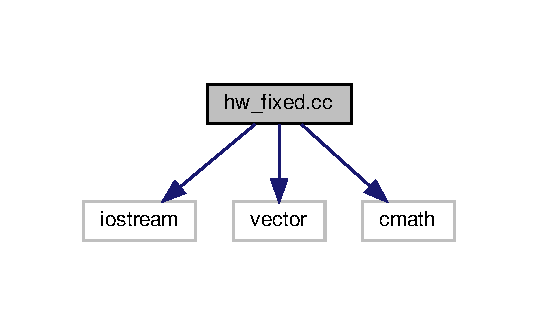
\includegraphics[width=258pt]{hw__fixed_8cc__incl}
\end{center}
\end{figure}
\subsection*{Functions}
\begin{DoxyCompactItemize}
\item 
double \hyperlink{hw__fixed_8cc_a9cfdbe00bb990c14c3a9e59a7dbbc974}{deviation} (int $\ast$a, int n)
\begin{DoxyCompactList}\small\item\em This function is to calculate standard deviation. \end{DoxyCompactList}\end{DoxyCompactItemize}


\subsection{Detailed Description}
! 

\subsection{Function Documentation}
\mbox{\Hypertarget{hw__fixed_8cc_a9cfdbe00bb990c14c3a9e59a7dbbc974}\label{hw__fixed_8cc_a9cfdbe00bb990c14c3a9e59a7dbbc974}} 
\index{hw\+\_\+fixed.\+cc@{hw\+\_\+fixed.\+cc}!deviation@{deviation}}
\index{deviation@{deviation}!hw\+\_\+fixed.\+cc@{hw\+\_\+fixed.\+cc}}
\subsubsection{\texorpdfstring{deviation()}{deviation()}}
{\footnotesize\ttfamily double deviation (\begin{DoxyParamCaption}\item[{int $\ast$}]{a,  }\item[{int}]{n }\end{DoxyParamCaption})}



This function is to calculate standard deviation. 


\begin{DoxyParams}{Parameters}
{\em a} & This variable is for the array of integers \\
\hline
{\em n} & This variable is the number of integers in the array \\
\hline
\end{DoxyParams}
\begin{DoxyReturn}{Returns}
This function returns the standard deviation of the integers in the array 
\end{DoxyReturn}


Definition at line 22 of file hw\+\_\+fixed.\+cc.


\begin{DoxyCode}
23 \{
24     \textcolor{keywordtype}{int} sum;
25     
26     \textcolor{keywordflow}{for}(\textcolor{keywordtype}{size\_t} i = 0; i <= n-1; i++)
27     \{
28         sum += a[i];
29     \} 
30     
31     \textcolor{keywordtype}{double} mean = sum /= (n-1);
32     \textcolor{keywordtype}{double} stddev = 0;
33     
34     \textcolor{keywordflow}{for}(\textcolor{keywordtype}{size\_t} i = 0; i <= n-2; i++)
35     \{
36         stddev += (a[i] - mean) * (a[i] - mean); 
37     \}
38     
39     stddev /= (n-1);
40     
41     \textcolor{keywordflow}{if}( stddev == 0)
42         std::cout << \textcolor{stringliteral}{"Sigma is zero."} << std::endl;
43     \textcolor{keywordflow}{return} sqrt(stddev);
44 \}
\end{DoxyCode}

%--- End generated contents ---

% Index
\backmatter
\newpage
\phantomsection
\clearemptydoublepage
\addcontentsline{toc}{chapter}{Index}
\printindex

\end{document}
